\documentclass{article}

\usepackage{microtype}
\usepackage{amsmath}
\usepackage{enumitem}
\usepackage{etoolbox}
\usepackage[svgnames]{xcolor}
\usepackage{pgfplots}
\usepackage{tikz}
\usepackage{tikz-3dplot}
\usepackage[letterpaper, bottom=100pt]{geometry}
\usepackage{physics}
\usepackage{float}

\usepgfplotslibrary{fillbetween}
\usetikzlibrary{calc}
\pgfplotsset{compat=newest}

\newcommand{\diff}[1]{\frac{#1}{dt}}
\newcommand{\vel}{\mathrm{v}}
\newcommand{\x}{\mathrm{x}}
\newcommand{\inter}{\int_{t_1}^{t_2}}
\newcommand{\tvert}{\biggr\rvert_{t_1}^{t_2}}
\newcommand{\derv}{\frac{\mathrm{d}}{\mathrm{d}t}}
\newcommand{\subx}[1]{\mathrm{\bf #1}_x}
\newcommand{\suby}[1]{\mathrm{\bf #1}_y}
\newcommand{\subz}[1]{\mathrm{\bf #1}_z}
\newcommand{\vect}[1]{(\subx{#1}, \suby{#1}, \subz{#1})}

\patchcmd\subequations
 {\theparentequation\alph{equation}}
 {\subequationsformat}
 {}{}

\newcommand{\subequationsformat}{\theparentequation.\arabic{equation}}

\author{Laith}
\title{Vectors and 3-Dimensional Space}
\date{1/30/2023}

\begin{document}
\maketitle
\section{Visualizing a 3D Space}
Objects can move in 3 ways with respect to a position, and \textbf{vectors} are used to
represent this. Vectors include both a direction and a distance.
\begin{figure}[H]
\begin{center}
\begin{tikzpicture}
\tdplotsetmaincoords{60}{110};
\pgfsetxvec{\pgfpoint{0.866cm}{-.5cm}};
\pgfsetyvec{\pgfpoint{0cm}{1cm}};
\pgfsetzvec{\pgfpoint{-.866cm}{-.5cm}};

\draw[->, color=green] (0, 0, 0) -- (3, 0, 0) node[anchor=west] {X};
\draw[->, color=blue] (0, 0, 0) -- (0, 3, 0) node[anchor=south] {Y};
\draw[->, color=red] (0, 0, 0) -- (0, 0, 3) node[anchor=north east] {Z};
\end{tikzpicture}
\end{center}
\end{figure}

\begin{figure}[H]
\begin{center}
\begin{tikzpicture}[scale=0.75]
\tdplotsetmaincoords{60}{110};
\pgfsetxvec{\pgfpoint{0.866cm}{-.5cm}};
\pgfsetyvec{\pgfpoint{0cm}{1cm}};
\pgfsetzvec{\pgfpoint{-.866cm}{-.5cm}};

\draw[->, color=green] (0, 0, 0) -- (3, 0, 0) node[anchor=west] {X};
\draw[->, color=blue] (0, 0, 0) -- (0, 3, 0) node[anchor=south] {Y};
\draw[->, color=red] (0, 0, 0) -- (0, 0, 3) node[anchor=north east] {Z};

\draw[->, color=black] (0, 0, 0) -- (1, 4, 0) node (a) {};
\draw[->, color=black] (0, 0, 0) -- (-1, 4, 0) node (b) {};
\draw[<->, color=gray] (a) -- (b) node[above] {$\Delta x$};

\draw[->, color=black] (0, 0, 0) -- (4, 1, 0) node (a) {};
\draw[->, color=black] (0, 0, 0) -- (4, -1, 0) node (b) {};
\draw[<->, color=gray] (a) -- (b) node[right] {$\Delta y$};

\draw[->] (0, 0, 0) -- (-4, 0, -1) node (a) {};
\draw[->] (0, 0, 0) -- (-4, 0, 1) node (b) {};
\draw[<->, color=gray] (a) -- (b) node[above, yshift=3] {$\Delta z$};
\end{tikzpicture}
\end{center}
\end{figure}

\newpage
\noindent In a 3D space, we have a new $z$ axis, thus our coordinates will include a new variable along this axis:
\[(x,\,y,\,z)\]
$x$ will represent our horizontal position, $y$ will represent our vertical position, and $z$ will represent our side-to-side position. 
With this in mind, displacement in a 3D space can be calculated as so:
\[\Delta \va{R} = (x-x_1,\, y-y_1,\, z-z_1)\]
Average velocity in a 3D space can be calculated as so:
\[\va{v} = (\frac{x-x_1}{\Delta t},\, \frac{y-y_1}{\Delta t},\, \frac{z-z_1}{\Delta t}) \]
If we want to obtain instantaneous velocity, we need to differentiate with respect to our
$x$, $y$, and $z$ positions:
\[\va{v}(t) = \va{R}'(t) = (\x'(t),\, \mathrm{y}'(t),\, \mathrm{z}'(t))\]

{\noindent \small I recommend returning to this section after reading the next section \textbf{Vectors}.}

\newpage
\section{Vectors}
Mathematically, vectors are represented as a variable
with an arrow on-top of it:
\[\va{a}\]
Above, we have a vector named \textbf{a}. This vector has \textbf{4} components, or parts:
\begin{align*}
    & \textbf{a} = \text{magnitude (distance)} \\
    & \textbf{a}_x = \text{x distance} \\
    & \textbf{a}_y = \text{y distance} \\
    & \textbf{a}_z = \text{z distance}
\end{align*}
The $x,\,y,$ and $z$ components are usually written like this:
\[ (\textbf{a}_x, \, \textbf{a}_y, \, \textbf{a}_z) \]
Vectors can represent different types of change. Three types of vectors are \textbf{displacement}, \textbf{velocity}, and \textbf{acceleration},
with displacement being the simplest to grasp. 
Vectors can be drawn, and below is a figure of displacement vectors:
\begin{figure}[H]
    \begin{center}
        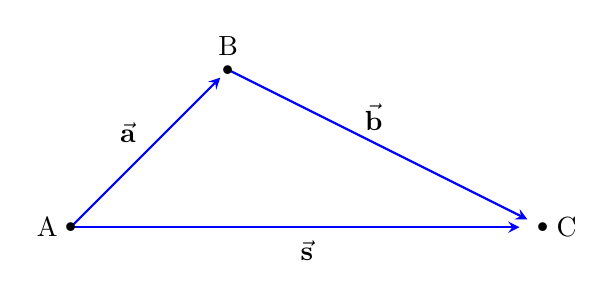
\begin{tikzpicture}[scale=2]

            \coordinate (A) at (0, 0) ; 
            \coordinate (B) at (1, 1) ; 
            \coordinate (C) at (3, 0) ; 

            \draw[-stealth, thick, color=blue] (A) -- ($(A)!.95!(B)$);
            \draw[-stealth, thick, color=blue] (B) -- ($(B)!.95!(C)$);
            \draw[-stealth, thick, color=blue] (A) -- ($(A)!.95!(C)$);

            \node[scale=3] at (A) {.};
            \node[left of=A, xshift=20] {A};
            \node[scale=3] at (B) {.};
            \node[above of=B, yshift=-20] {B};
            \node[scale=3] at (C) {.};
            \node[right of=C, xshift=-20] {C};

            \coordinate (a) at ($(A)!.60!(B)$);
            \node[left of=a, xshift=15] {$\va{a}$};
            \coordinate (b) at ($(B)!.30!(C)$);
            \node[right of=b, xshift=-10] {$\va{b}$};
            \coordinate (c) at ($(C)!.50!(A)$);
            \node[below of=c, yshift=20] {$\va{s}$};

        \end{tikzpicture}
    \end{center}
\end{figure}
\noindent Vectors can actually be added, so with the case of $\va{a} \text{   and   } \va{b}$,
their sum would be vector $\va{s}$. Keep in mind that vectors have $x,\,y,$ and $z$ components, so
the sum of two or more vectors cannot be just the sum of their lengths.

We geometrically added vectors in the above figure, but vector sums can also be calculated,
and we do so by adding component by component:
\begin{gather*}
    \va{a}+\va{b}=\va{s} \\ 
    \intertext{\centering In order to add vectors $\va{a}$ and $\va{b}$, we first need to break them up into their components.}
    \vect{a}+\vect{b}=\vect{s} \\
    \intertext{\centering Now, we can essentially add by like terms:}
    \subx{s} = \subx{a} + \subx{b} \\
    \suby{s} = \suby{a} + \suby{b} \\
    \subz{s} = \subz{a} + \subz{b} \\
    \intertext{\centering So naturally, the vector sum would look like this:}
    \va{s} = (\subx{a} + \subx{b},\, \suby{a} + \suby{b},\, \subz{a} + \subz{b})
\end{gather*} 
\newpage
The length, or magnitude, of a vector can be calculated with the below formula:
\[\va{a} = \sqrt{{\subx{a}}^2+{\suby{a}}^2+{\subz{a}}^2}\]

\end{document}